%Einleitung.tex
%
\chapter{Introduction}
\section{Motivation}
\subsection{Performance \& Testing}
Performance of software is the process of analyzing a given program and reacting to problems that may or may not occur during runtime. The less unexpected problems emerge, the better the performance of that software\cite{8432081}. 
To make sure fewer problems occur, one could adopt methods like the \textit{Software Performance Engineering}, which uses quantitative techniques to identify designs with lesser flaws and so spare the developers significant time in their implementation\cite{4299916}. An idealistic scenario would be, if the product would have no flaws at all. But as many know, perfectness is hard to achieve, even harder if people keep developing the product. Even if the outcome may be perfect at a certain point in time, the continuous development will certainly show incompatibilities with the functional state of the product.
\begin{center}
	\say{If anything can go wrong, it will}
	\begin{flushright}
		\textit{Murphy's law}
	\end{flushright}
\end{center}
To avoid the release of a defect product and support the \textit{SPE} approach, one needs to implement additional tests, because bugs can appear even after deployment as the development process advances.\\
Testing in the IT-Branch is an approach with the main goal of finding bugs in a software program or application. These bugs refer to errors or faults and can occur because of a bad commands sequence specified in the program's source code or incompatibility of other member of the program. This can often occur especially when the \dq amount of libraries are high and the mutual dependencies complex\dq{}\cite{7302456}. A successful test can be achieved when its main requirements are met. Some examples would be the execution on different environments, time constraints or delivering expected outputs for randomly chosen inputs. Conditions are set by the tester and may vary. These are frequently chosen based on user cases and logical expectations.\newpage
\subsection{General}
Most companies put a lot of effort in delivering high performance products to their customers. In order to do so, each of them test their gadgets, machines or software for possible failure scenarios. The test phases usually take place before the release of a new product or the deployment of an update that brings new features to an existing product.\\
Now-a-days tests are being fully automated, which decreases the failure possibility that can happen because of human errors\cite{8389562}. Unfortunately the creation of fully automated tests is not as easy as it may sound. Many testing developers know the struggle of finding the right tools for the job without filling their projects with unnecessary dependencies that will overload the program and occupy valuable memory.
\begin{center}
	\say{As ironic as it seems, the challenge of a tester is to test as little as possible. Test less, but test smarter}
	\begin{flushright}
		\textit{Federico Teldo, Co-Founder Abstracta US}
	\end{flushright}
\end{center}
Additionally the problem enhances when a company reaches a certain size with a significant number of customers, which tend to run the product on different machines and architectures. In order to keep their customers, producers need to adapt their products to support newer or older machines. This makes software analysis even more difficult because of the increasing complexity, which comes with different systems. For this reason many companies dedicated themselves to creating programs that focus only on software examination and fixing bugs that may occur during an analysis	. In time a new trend has been created with demands so high that rapidly developed itself into a new market section.\\
\section{Growing markets}
For the last decade the software testing market has been developing and now it has grown so big that it would be foolish to ignore it. According to \dq Global Market Insights\dq{} the testing software market has grown up to 40 billion dollars by the end of 2020 and is predicted to grow up to 60 billion dollars in the next 6 years.\cite{GMI}\\
\textit{\dq People may lie, but number don't\dq}. Multiple scientific papers and studies enforce this statement with different statistics of industries, which started adapting and reacting to this trend using the model \dq EaaS \dq{} which stands for \dq Everything as a service\dq{} and created \dq Testing as a Service\dq{}(TaaS). With this model customers not only pay for the current state of a product, but also for a service subscription, where they get updates and new features for the specific product and additional support from the company. The advantages that benefit the customer are set by the company for each of their subscription. (The basic rule is that you get more accurate results if you pay more). This service usually targets three groups: Developers, End Users and Certification Services.\cite{10.1145/1807128.1807153} 
\begin{figure}[htbp]
	\centering
	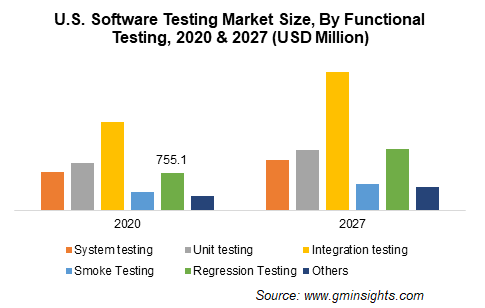
\includegraphics[width=0.80\textwidth]{../figures/einleitung/US_marketsize.png}
	\caption{US Software Market Size\cite{GMI}}
	\label{US_marketsize_graph}
\end{figure}

\subsection{The costs of perfection}
People often tend to overlook costs of testing tasks that are insignificant in comparison to the total price of the project. However if these costs are reoccuring, their total price can go up to 40\% of the total project's costs\cite{8822082}.\\
There are two common ways to cope with this problem. First, one could use a third party software that specializes in testing other companies's software. This has its advantages, because the tests are already written to work on most compilers for a majority of programming languages. The bad part though, is the pricing, which may or may not be a problem for a company (depending on its size) and additional privacy issues, because we can't \dq look behind the curtains\dq{} of a compiled software, therefore we cannot tell what kind of data the program stores about the user or whom may it send it to.\\
The second way it would be to let the company's developers test themselves. This method proves often quite efficient, because they are the ones who programmed the software and therefore the best candidates to repair possible bugs and the company is not exposed to any additional privacy risks. However the whole process needs to be led by someone experienced enough to correctly organize it for the current tasks,but also for the future ones. Unfortunately when people test internally, additional costs appear. At the begging it may be more expensive than buying a testing software, but in the long run will be cheaper as the testing process gets more and more refined. That amount of money covers not only for direct testing, which includes the staff, system and program testing, resources, computer time, etc. , but also for indirect testing, which refers to actions that take place because of poor direct testing, like rewriting code, additional analysis meetings or debugging.\\
It was proven that the cost of finding an error is about \$50 on average \cite{10.1145/1010773.1010774}, and is said that fixing an error after the software was released is four times more expensive than compared to if it was found during the testing phase.\cite{10.1007/978-981-10-8848-3_46} To avoid these financial expenses, companies can train their developers to consider failure scenarios of the product early in the development stage.

\subsection{Common approaches}
In order to deliver a defect-free product, managers create testing strategies.
To develop the most suitable strategy, they must identify the key components for it. These can be identified mostly by answering the following questions adapted from \cite{10.1007/978-981-10-8848-3_46}:
\begin{enumerate}
	\item Is the objective clear specified?
	\item What tools will be used?
	\item Is the system fully/partially automated?
	\item How will the test benefit the project?
\end{enumerate}
Additionally, the results and procedures need to be recorded in order to make testing phases smoother, because the same errors may occur in the future.
% enumarate:
% weitere heruasforderung - unterschiedliche OS mit teilweise spezifischen testanforderungen
% diese äußern sich vor allem im Perfromancebetrachtungen -> zusätzliche Aufwände und Herausforderungen
% wenn das profitable ist, dann sollte das auf alle OS laufbar sein um den ganzen Markt zu erreichen
% bedarf eines Tools das auf alle OS anwendbar ist und vergleichbare Ergebnisse zeigt
% 
\section{Benchmarking}
In addition to testing, companies also have the desire to reach as many customers as possible. In order to do that many tend to create benchmarks that show the product's superiority in comparison to other products that fulfill the same task and reduce production costs.\\
According to the \textit{Standard Performance Evaluation Corporation} (short \textit{SPEC}), a benchmark is a \dq test, or set of tests, designed to compare the performance of one computer system against the performance of others\dq{}\cite{spec-benchmark}. A method developed by \textit{Infineon Technologies AG} ,written by Lukas Klaus, explains \dq The intention [...] [to] keep cost of test constant relative to overall cost of goods sold\dq{}. Klaus mention that once the yearly costs of production were established, once can come up with a financial plan that compares the manufacturing expenses with the \dq hypothetical best case if all products in question were at benchmark performance\dq{}. The method can additionally create in an indicator, which can be calculated by dividing test costs by the revenue of sold goods\cite{4221595}. This can be used to help decisions on which part is worth improving in order to create the best product while maximizing customer satisfaction.\\  
This leads to the question \dq What makes a good benchmark?\dq{}.\\
A paper written by Maya Daneva of Institute of Business Information Systems at the University Of Saarland answered this explaining the designs and usage of software benchmarking. According to her the targets of this approach can be classified in different classes of organizations with different set of goals. The most relevant for this thesis are software developers, distributors, testing laboratories and researchers, as well as certifications offices, academic intuitions and independent benchmarking companies. For a well made benchmark, Daneva introduced six crucial criterias\cite{Daneva1995}:
\begin{enumerate}
	\item Pertinence 
	\item Functional coverage   
	\item Understandability 
	\item Ease of use  
	\item Interpretability
	\item Reproducibility
\end{enumerate}    
When creating the benchmark one would try to achieve perfectness in every aspect of each criteria, but the reality often tends to disappoint our expectations. To explain this in detail you could think about these criteria as a hexagon with six angles. When the developer tries to implement one side of the hexagon to perfection he often would have to give up on other sides as pictured in Figure \ref{hexagon_criterias}. Most of the times one needs to identify the most important aspect that matters the most to him and choose it over less relevant ones (though this doesn't have to be always the case)
\begin{figure}[htbp]
	\centering
	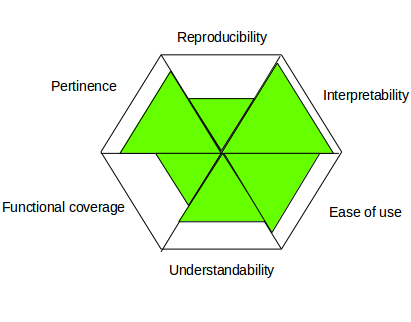
\includegraphics[width=0.6\textwidth]{../figures/einleitung/hexagon.png}
	\caption{Hexagon of criteria}
	\label{hexagon_criterias}
\end{figure}
\\In order to generate reliable statistics, the creator also needs to considerate the additional workload the benchmark is creating and to differentiate between the actual strains put on the system by the application at hand and those created by the benchmark. 
\subsection{Workload}
The definition for workload varies from field to field. In the IT-branch it is defined as a unit of measure for your CPU (mostly in \%). This tells the user how well his system can handle the number of current running processes.\\
Workloads are made out of two parts: the executable part and the non-executable part. The executable part refers to code that is being executed when an application software is being executed. The non-executable part refers to the workload produced in order for the executable part to have \dq a well-defined and reproducible manner\dq{}. One can also differentiate between natural and artificial workload. Natural workloads are produced by software executing useful tasks and benchmarks that deliver statistics based on such workloads are also called \textit{natural benchmarks}. Artificial workloads however are generated by code that tries to mimic real workload (most time irrelevant code like the incrementation of a variable in a loop). Most benchmarks often implement artificial workloads ,because they \dq allow[ing] one to measure the limits of a system, or a selected part of it, unde different configurations and workloads\dq{} while natural ones often tend to need user input, cannot be entirely reproduced and often unfair to other processes,based on the application's high optimization for the software to run as smooth as possible, which can put pressure on the system's hardware\cite{Kounev2020}. When it comes to performance both artificial and real workloads are similar. Additionally good benchmarks that implement artificial workload need to prevent critical situations when the user might overload the system and bring it to a halt, which for most cases is undesirable.\\
Many systems calculate their workload over a defined period of time. The following example explains how one system can estimate the workload of a simple application. Let's say a user starts a calculator program at time $\mathrm{t}_0$ = 0. The application will finish initializing a GUI at time $\mathrm{t}_{wait}$ = 2s and then an interactive visual window will appear, which will wait for the user to enter some equation.
After the equation was typed at $\mathrm{t}_{input}$ = 5s and the \dq Enter\dq{}-key was pressed, the application proceeds calculating and delivers the answer at $\mathrm{t}_{done}$ = 6s. So the CPU-time of the application is 3s(GUI initialization and calculation time). In order to get its workload the system has to divide this time by the time the system needed for the whole process and multiply it by one hundred to have the result as percentage:\\
\begin{equation}
workload =  \frac{3s(\mathrm{t}_{wait}+\mathrm{t}_{calc})}{6s}*100
\end{equation}\\
A detailed explanation on how to get the values of process and system specific times will follow in \ref{system-methods}.
\section{Obective}
The purpose of this thesis is the development, implementation and testing of a Library for C++ applications that creates an artificial workload and delivers system independent statistics based on multi-threading. This will allow developers to implement their own stress tests and run simulations with different workloads, process priorities and scheduling, which can be used in different manners to achieve real-time applications and create benchmarks for each new product. %These could be later automatized by using programs like \href{https://www.jenkins.io/}{Jenkins}\cite{Jenkins} or \href{https://about.gitlab.com/}{Gitlab}\cite{GitLab}.

%\section{Advantages and Disadvantages}
%\subsection{Pros}
%\begin{enumerate}
%	\item No additional expenses for third party software or subscriptions
%	\item Can be directly added to the source code, which makes testing easy
%	\item No external influence from the browser(ads) or internet connection, allowing efficient testing even offline
%	\item Allows the creation of tests based on user experience 
%	\item Companies don't have to give their data 
%\end{enumerate}

%\subsection{Cons}
%\begin{enumerate}
%	\item Tests don't come already prepared
%	\item Developers have to add the source code to their build system or add the build files(CMakeLists.txt) to their own (if they already use CMake)
%\end{enumerate}
%\section{Summary}
%With this library a company can save money, improve their product based on user feedback or create an internet independent test system for very minimal effort and a product specific benchmark.